\section{Inpainting}

\begin{frame}{Inpainting}
\begin{block}{Denière partie de l'algorithme}
Appliquer le masque $\Phi$ extrait et remplir les \og trous\fg - problématique d'\emph{inpainting}.
\end{block}
\begin{description}
\item[Inpainting par régularisation variationnelle. ]Retrouve une image par le problème d'optimisation - norme TV ou Sobolev \emph{e.g.} :
\begin{equation}
f^* = \arg \min E(f) = \|\nabla f \|^2 \text{ s.c. } \Phi(f) = y
\end{equation}

\item[Inpainting par régularisation parcimonieuse. ]Passe par une représentation $a = (a_m)_m$ - base d'ondelettes par exemple - parcimonieuse et résout : 
\begin{equation}
a^* \in \arg \min_a \frac{1}{2} \| y - \Phi \Psi a \|^2 + \lambda J(a)
\end{equation}
\end{description}
\end{frame}


\begin{frame}{Inpainting}
\begin{figure}
\centering
\begin{tabular}{ccc}
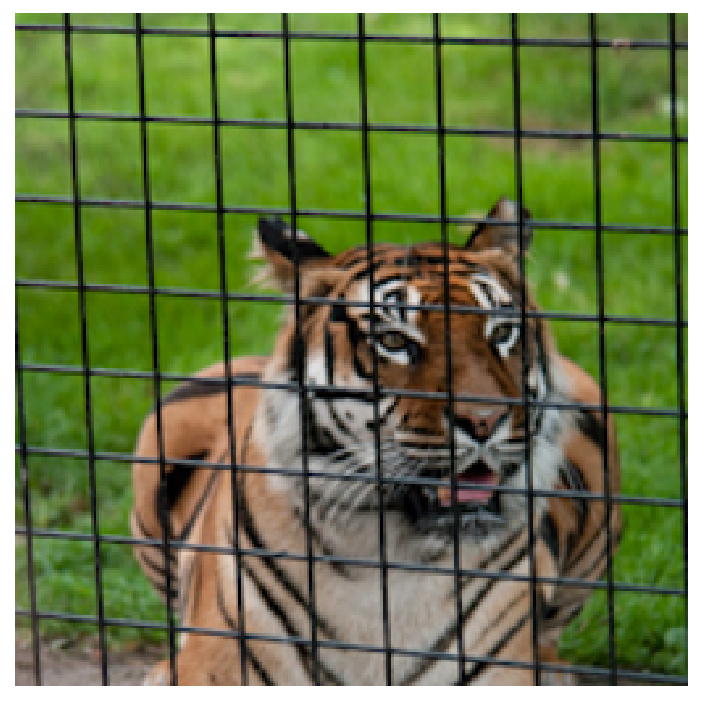
\includegraphics[width = .3\columnwidth]{fig/tigre_initial.png} &
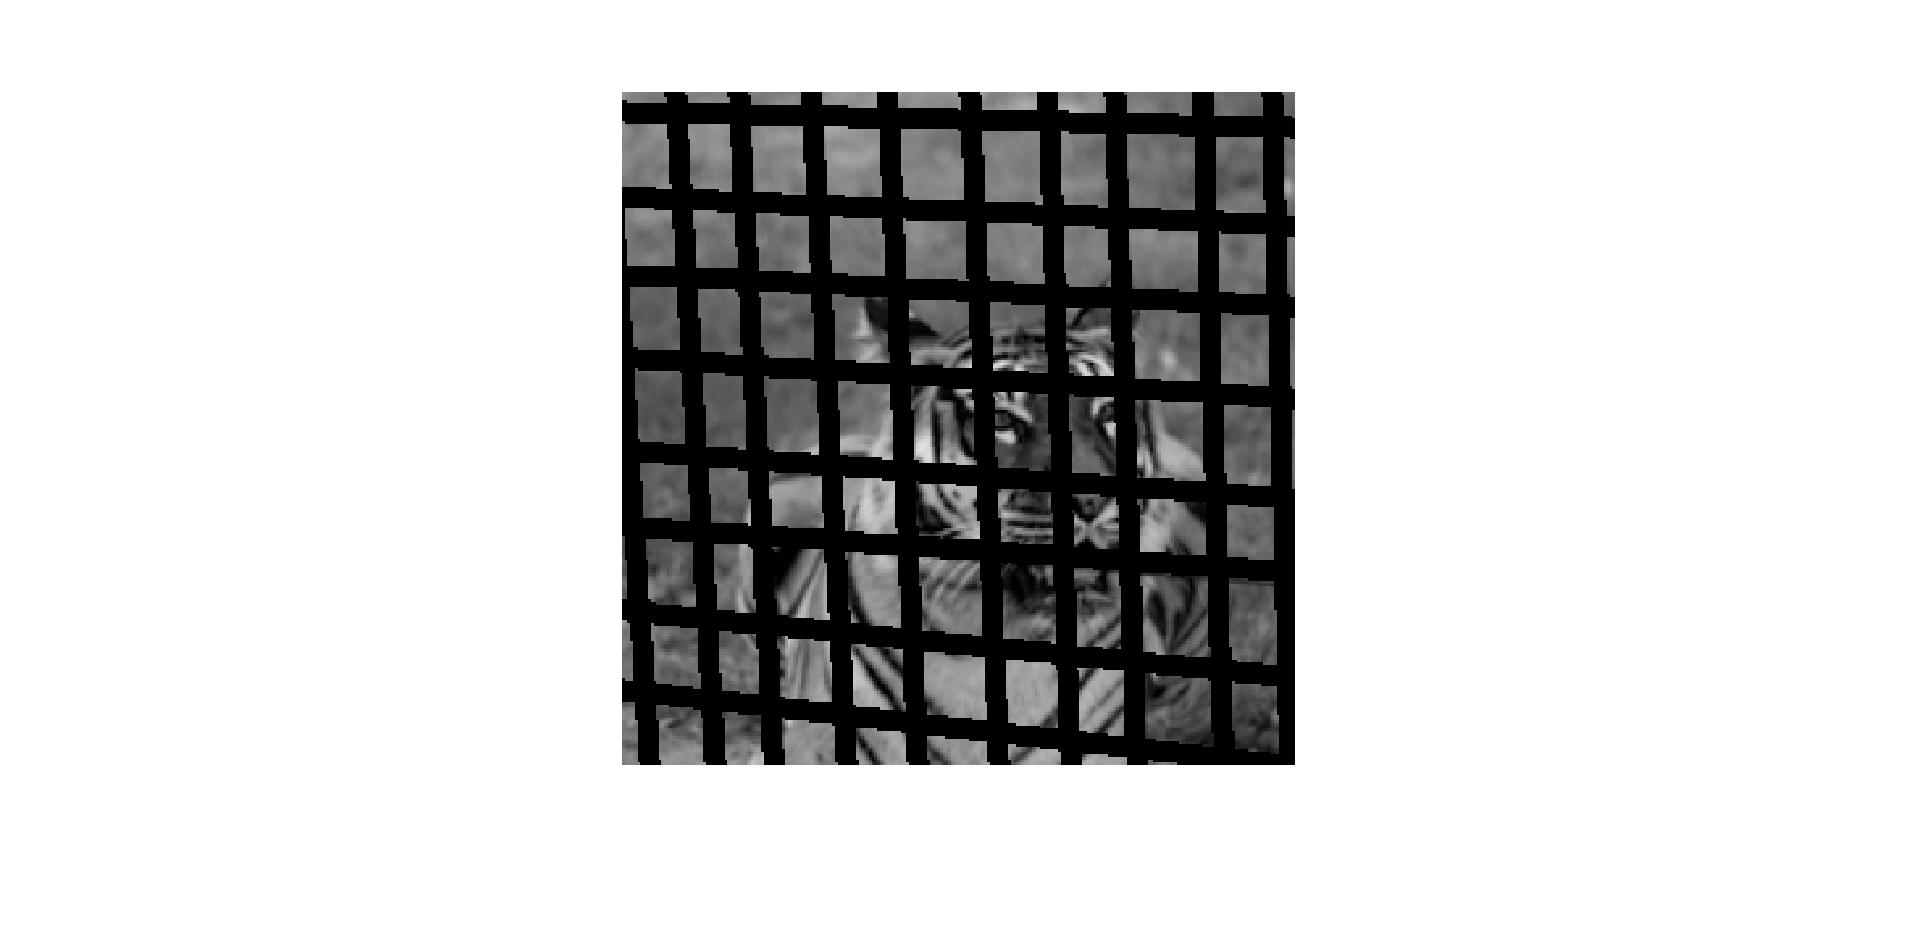
\includegraphics[width = .3\columnwidth]{fig/tigre_masque.png} &
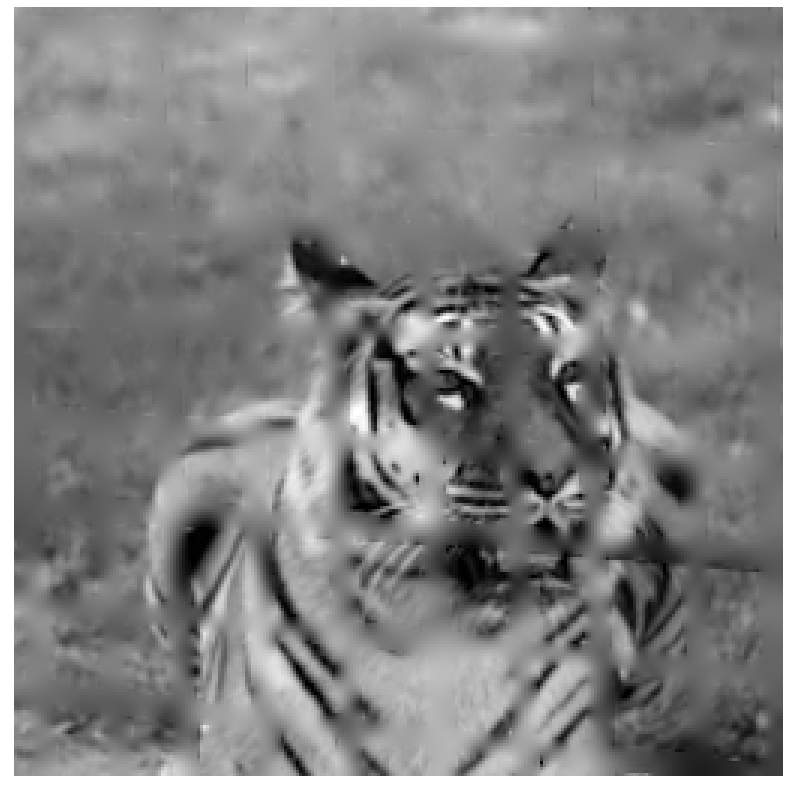
\includegraphics[width = .3\columnwidth]{fig/tigre_inpainting.png} \\
\end{tabular}
\caption{Processus d'\emph{inpainting} sur l'image du tigre.}
\end{figure}
\end{frame}
